\documentclass{article}
\usepackage{listings, xcolor, graphicx, inconsolata, amsmath}
\setlength{\parindent}{0pt}

\definecolor{lgray}{rgb}{0.95, 0.95, 0.95}
\definecolor{lgray2}{rgb}{0.75, 0.75, 0.75}

\lstset{
  language=C++,
  aboveskip=10pt,
  belowskip=10pt,
  frame=leftline,
  xleftmargin=15pt,
  framexleftmargin=20pt,
  breaklines=true,
  basicstyle=\small,
  showstringspaces=false,
  backgroundcolor=\color{lgray},
  rulecolor=\color{lgray2},
  basicstyle=\ttfamily\footnotesize,
  keywordstyle=\color{blue},
  stringstyle=\color{red},
  commentstyle=\color{green},
  numbers=left,               
  numberstyle=\tiny\color{gray},
  stepnumber=1
}

\title{CS135; 1D Arrays and Strings}
\author{Gael Zarco}
\date{\today}

\begin{document}

\maketitle

\textbf{Structured Data Types} contain data where each item is a collection of
other data items.
\begin{itemize}
  \item Simple data structures are the building blocks of structured data types.
\end{itemize}

% SECTION 1 %
\section{Arrays}
An \textbf{Array} is a collection of a fixed number of components (also called
elements) all of the same data type and in contigous (adjacent) memory space. A
\textbf{One-Dimensional Array} is an array in which the components are arranged
in a list form.

\begin{lstlisting}[caption={1D Array Syntax}]
  dataType arrayName[intExp];

  // Example
  int list[5];    // Declared array 'list' of 10 elements
\end{lstlisting}

\texttt{intExp} specifies the number of components in the array and can be any
constant expression that evaluates to a positive integer. The Example above
delcares an array \texttt{list} of \textit{10} components.

\begin{itemize}
  \item The components are \texttt{list[0], list[1], ..., list[9]}.
  \item Declares a total of 10 variables
\end{itemize}

\begin{center}
    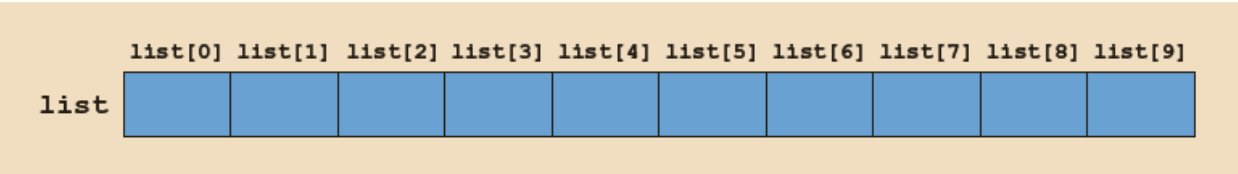
\includegraphics[width=0.9\textwidth]{1d-arr-vars.png}
\end{center}

\begin{lstlisting}[caption={1D Array Assignment}]
  list[5] = 34;
\end{lstlisting}

This expression stores \textit{34} in \texttt{list[5]}, which is the
\textit{sixth} component of the array \texttt{list}.

\begin{itemize}
  \item You can use \texttt{i} to index into an array.
  \begin {itemize}
    \item \texttt{list[i]}
  \end{itemize}
\end{itemize}

\begin{center}
    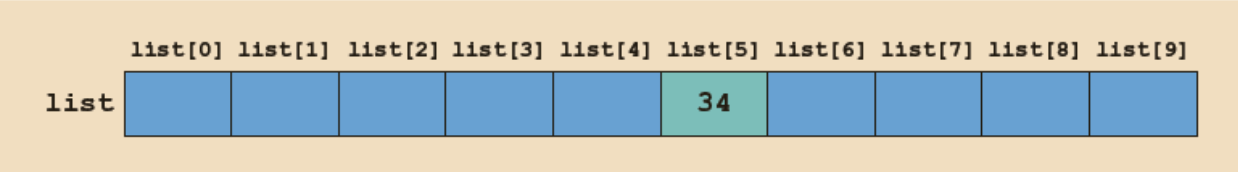
\includegraphics[width=0.9\textwidth]{1d-arr-var-assign.png}
\end{center}

\begin{lstlisting}[caption={1D Array Assignment Cont}]
  list[3] = 10;
  list[6] = 35;

  // Add the contents of list[3] and list[6] and store in list[5]
  list[5] = list[3] + list[6];
\end{lstlisting}

\begin{center}
    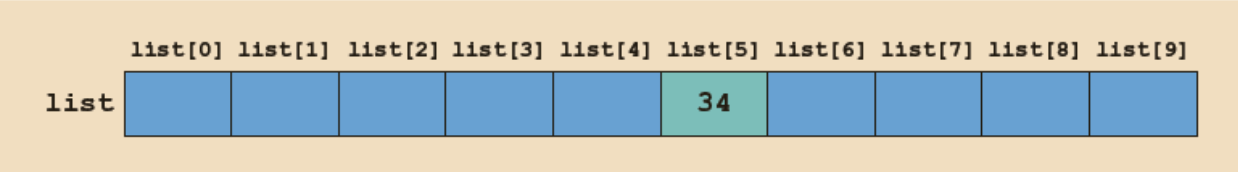
\includegraphics[width=0.9\textwidth]{1d-arr-var-assign.png}
\end{center}

% SECTION 1.1 %
\subsection{Processing One-Dimensional Arrays}

\begin{lstlisting}[caption={Read Data Into 1D Array}]
  for (i = 0; i < 10; i++)
    cin >> list[i];
\end{lstlisting}

\begin{lstlisting}[caption={Print Data From 1D Array}]
  for (i = 0; i < 10; i++)
    cout << list[i];
\end{lstlisting}

\begin{lstlisting}[caption={Find Sum \& Avg From 1D Array}]
  int sum = 0;
  int avg;

  for (i = 0; i < 10; i++)
    sum = sum + list[i]; 

  avg = sum / 10;
\end{lstlisting}

\begin{lstlisting}[caption={Find Largest Element in 1D Array}]
  int maxIdx = 0;

  for (int i = 1; i < 10; i++)
    if (list[maxIdx] < list[i])
      maxIdx = i;

  int largestInt = list[maxIdx];
\end{lstlisting}

% SECTION 1.2 %
\subsection{Array Index Out of Bounds}

\begin{lstlisting}[caption={Array Index Example}]
  double num[10];
  int i;
\end{lstlisting}

The component \texttt{num[i]} is \textit{valid} or \textbf{In Bounds} if
\texttt{index}:
\begin{itemize}
  \item $0 \leq \text{index} \leq \text{ARRAY\_SIZE} - 1$.
  \item \texttt{index} is not negative or greater than $\text{ARRAY\_SIZE} - 1$.
  \begin{itemize}
    \item It is \textbf{Out of Bounds} in this event.
    \item C++ does not check whether the index value is within range; this is
      the programmer's responsibility.
  \end{itemize}
\end{itemize}

% SECTION 1.3 %
\subsection{Array Initialization During Declaration}
An array can be initialized while being declared

\begin{lstlisting}[caption={Array Initialization Example}]
  double sales[5] = {12.25, 32.50, 16.90, 23, 45.68};

  // Not necessary to specify the size when initializing
  double sales[] = {12.25, 32.50, 16.90, 23, 45.68};
\end{lstlisting}

% SECTION 1.4 %
\subsection{Partial Initialization of Arrays During Declaration}

\begin{lstlisting}[caption={Partial Array Initialization}]
  int list[10] = {5, 6, 3};
\end{lstlisting}

The first three components of \texttt{list} are \texttt{list[0] = 5, list[1] =
6, list[2] = 3}, and the rest are set to the default of 0.

% SECTION 1.5 %
\subsection{Restrictions on Array Processing}
C++ does not allow \textbf{Aggregate Operations} on an array. Aggregate
operations on an array are any operations that manipulate the entire array as a single unit.

\begin{lstlisting}[caption={Illegal Aggregate Operation on Array}]
  int myList[5] = {0, 4, 8, 12, 16};
  int yourList[5];

  // illegal
  yourList = myList;
\end{lstlisting}

% SECTION 1.6 %
\subsection{Arrays as Parameters to Functions}
In C++, arrays are passed as parameters to functions by \textbf{Reference Only}.
You do \textbf{not} use the \texttt{\&} symbol when declaring an array as a
formal parameter.

\begin{lstlisting}[caption={Arrays as Formal Parameters}]
  void initialize(int list[], int listSize);
\end{lstlisting}

% SECTION 1.7 %
\subsection{Constant Arrays as Formal Parameters}
You can use \texttt{const} keyword in the declaration of a formal param to
prevent the function from changing the actual param.

\begin{lstlisting}[caption={Constant Arrays as Formal Parameters}]
  void foo(int x[], const int y[], int sizeX, int sizeY);
\end{lstlisting}

% SECTION 1.8 %
\subsection{Base Address of an Array and Array in Computer Memory}
The \textbf{Base Address} of an array is the address (memory location) of the
first array component.
\begin{itemize}
  \item In 1D arrays, the base address is list[0];
\end{itemize}

\begin{center}
  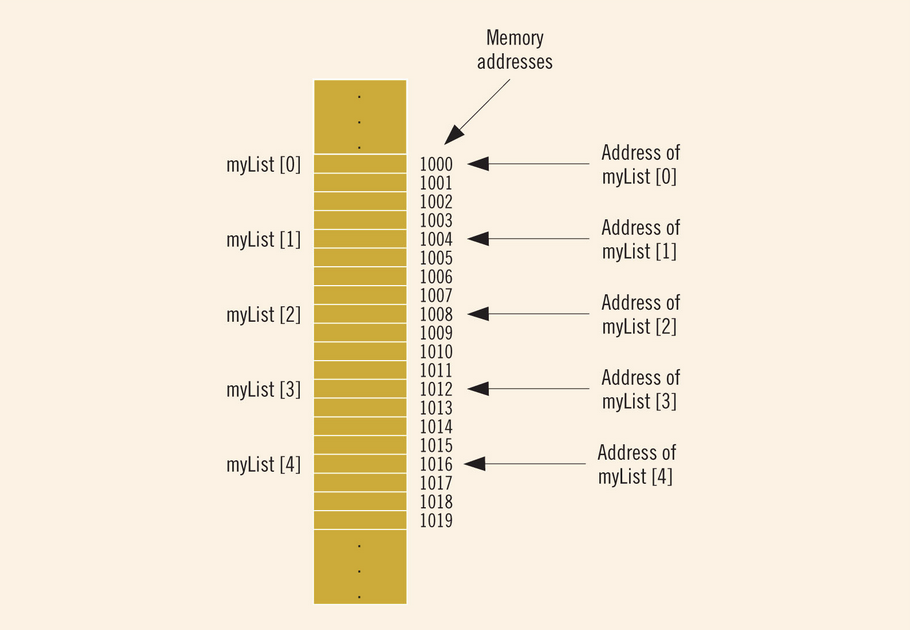
\includegraphics[width=0.9\textwidth]{arr-addy-com-mem.png}
\end{center}

% SECTION 1.9 %
\subsection{Functions Cannot Return a Value of the Type Array}
C++ does not allow functions to return a value of type array.

% SECTION 1.10 %
\subsection{Integral Data Type and Array Indices}
C++ allows any integral type to be used as an array index.

\begin{lstlisting}[caption={Improved Code Readability}]
  enum paintType { GREEN, RED, BLUE, BROWN, WHITE, ORANGE, YELLOW };
  double paintSale[7];

  paintSale[RED] = paintSale[RED] + 75.69;
\end{lstlisting}

% SECTION 1.11 %
\subsection{Other Ways to Declare Arrays}

\begin{lstlisting}[caption={Declaration Using Existing Variable}]
  const int NO_OF_STUDENTS = 20;
  int testScores[NO_OF_STUDENTS];
\end{lstlisting}

\begin{lstlisting}[caption={Declaration with \texttt{using}}]
  const int SIZE = 50;        // Line 1
  using list = double[SIZE];  // Line 2
  list yourList;              // Line 3
  list myList;                // Line 4
\end{lstlisting}

% SECTION 2 %
\section{Searching an Array for a Specific Item}
\textbf{Sequential Search} (\textit{linear search}):
\begin{enumerate}
  \item Searching a list for a given item, starting from the first element.
  \item Compare each element in the array with the value being searched.
  \item Continue to search until item is found or no more data is left. 
\end{enumerate}

\begin{lstlisting}[caption={Simple Array Search}]
  int seqSearch(const int list[], int listLength, int searchItem) {
    int  loc   = 0;
    bool found = false;

    while (loc < listLength && !found) {
      if (list[loc] == searchItem) {
        found = true;
      } else {
        ++loc;
      }
    }

    return found ? loc : -1;
  }
\end{lstlisting}

% SECTION 3 %
\section{Sorting}
\textbf{Selection Sort} is rearranging the list by selecting an element and
moving it to its proper position.

\begin{enumerate}
  \item Find the smallest element in the unsorted portion of the list.
  \item Move it to the top of the unsorted portion by swapping with current
    element.
  \item Start again with the rest of the list.
\end{enumerate}

\begin{center}
    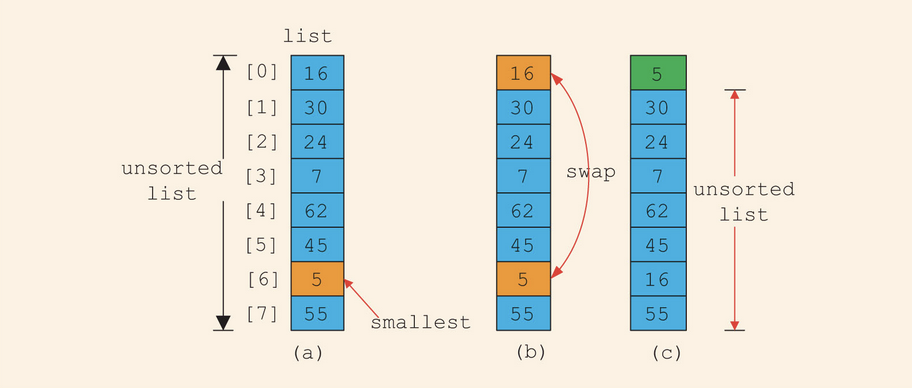
\includegraphics[width=0.9\textwidth]{1D-sel-sort.png}
\end{center}

% SECTION 4 %
\section{Auto Declaration and Range-Based \texttt{for} Loops}
Modern C++ allows for \textbf{Auto} declaration of variables
\begin{itemize}
  \item Data type does not need to be specified.
\end{itemize}

\begin{lstlisting}
  auto num = 15;
\end{lstlisting}

The compiler deduces \texttt{num} to be of type \texttt{int}.

\begin{lstlisting}[caption={Range-Based \texttt{for} Loop}]
  double list[25];
  double sum = 0;

  for (double num : list) {  // read as "for each num in list"
      sum += num;
  }
\end{lstlisting}

% SECTION 5 %
\section{C-Strings (Character Arrays)}
A \textbf{Character Array} is an array whose components are of type
\texttt{char}.

\begin{itemize}
  \item C-strings are \textit{null-terminated} (\texttt{'\\0'}) character arrays.
  \item Examples
    \begin{itemize}
      \item 'A' is the character A
      \item "A" is the C-string A
      \item \textit{Note}: "A" represents two characters. 'A' and \texttt{'\\0'}.
    \end{itemize}
\end{itemize}

\begin{lstlisting}[caption={C-String Declaration}]
  char name[16];
\end{lstlisting}

C-strings are null-terminated and \texttt{name} has 16 components, the largest
string it can store has 15 characters. If you store a string whose length is
less than the array size, the last components are unused.

\begin{lstlisting}[caption={Omitting Size of Array During Initialization}]
  char name[] = "John";
\end{lstlisting}

Declares an array of length \textit{5} and stores the C-string "John" in the
array. Useful \texttt{string} functions:

\begin{itemize}
  \item \texttt{strcopy}
  \item \texttt{strncpy}
  \item \texttt{strcmp}
  \item \texttt{strlen}
\end{itemize}

% SECTION 5.1 %
\subsection{String Comparison}
C-Strings are compared character by character using the collating system
sequence. Use the \texttt{strcmp} function to compare strings.

\vspace{8pt}

If using ASCII char set:
\begin{itemize}
  \item "Air" < "Boat"
  \item "Air" < "An"
  \item "Bill" < "Billy"
  \item "Hello" < "hello"
\end{itemize}

% SECTION 5.2 %
\subsection{Reading and Writing Strings}
Most array rules apply to C-strings (which are \texttt{char} arrays). However,
C++ \textbf{DOES} allow aggregate ops for the input and output of C-strings.


% SECTION 5.3 %
\subsection{String Input}
\begin{lstlisting}[caption={String Input Example}]
  cin >> name;
\end{lstlisting}

Stores the next input C-string into \texttt{name}.

\begin{lstlisting}[caption={Read Strings with Blanks with \texttt{get}}]
  cin.get(str, m + 1);
\end{lstlisting}

\begin{itemize}
  \item When executed, stores the next \texttt{m} characters into \texttt{str}, but the
newline character is not stored.
  \item If input string has fewer than \texttt{m} characters, reading stops at
    newline character.
\end{itemize}

% SECTION 5.4 %
\subsection{String Output}
\begin{lstlisting}[caption={String Output Example}]
  cout << name;
\end{lstlisting}

\begin{itemize}
  \item \texttt{<<} continues to write the contents of \texttt{name} until it
    finds a \texttt{null} character.
  \item If \texttt{name} does not contain a \texttt{null} character, then
    strange output may occur as it will continue to output data from memory until a
    \texttt{null} character is found.
\end{itemize}


% SECTION 5.5 %
\subsection{\texttt{string} Type and Input/Output Files}
Argument to open function must be a null-terminated string (a C-string).

\begin{itemize}
  \item If using a string var for the name of an I/O file, the value must first
    be converted to a C-string before calling \texttt{open}.
  \item Use the \texttt{c\_str} function to convert.
\end{itemize}

\begin{lstlisting}[caption={\texttt{c\_str} Syntax}]
  strVar.c\_str();
\end{lstlisting}

Where \texttt{strVar} is a variable of type \texttt{string}.

\end{document}
